\documentclass[letterpaper,12pt]{article}
\usepackage{tabularx} % extra features for tabular environment
\usepackage{amsmath}  % improve math presentation
\usepackage{float}
\usepackage{pdfpages}


\usepackage{graphicx} % takes care of graphic including machinery
\graphicspath{ {./figures/} }
%\usepackage[margin=1in,letterpaper]{geometry} % decreases margins
%\usepackage{cite} % takes care of citations
\usepackage[final]{hyperref} % adds hyper links inside the generated pdf file
\hypersetup{
	colorlinks=true,       % false: boxed links; true: colored links
	linkcolor=blue,        % color of internal links
	citecolor=blue,        % color of links to bibliography
	filecolor=magenta,     % color of file links
	urlcolor =blue         
}
\usepackage[margin = 1in,headsep=0.5cm,headheight=2cm,letterpaper]{geometry} 

\usepackage{fancyhdr}
\pagestyle{fancy}
\lhead{Student 1 : Ahmet Akman 2442366 \\ Student 2: Yusuf Toprak Yıldıran 2444149 \\ Assistant: Onur Selim Kılıç}
\rhead{Date: \today \\ Group: Wednesday Morning - 5} 
%\cfoot{center of the footer!}
\renewcommand{\headrulewidth}{0.1pt}



\begin{document}
\thispagestyle{empty}

\title{Spring 2022 EE214 Project Work  \protect\\ PreliminaryWork }
\author{Ahmet Akman 2442366 \protect\\ Yusuf Toprak Yıldıran 2444149 \protect\\ Assistant: Onur Selim Kılıç}
\date{\today}
\maketitle
\tableofcontents
%\begin{abstract}
%abstract
%\end{abstract}
\section{Introduction}
\section{Experimental Results and Discussion}
The results of the experiment are discussed in the following steps.
%
\subsection{Transmitter Unit}
\subsection{Receiver Unit}
In this part a receiver needed to be designed. So, let us first define the design requirements.
\begin{itemize}
    \item The receiver should be able extract the desired signal amongst the signals with 12 different frequencies.
    \item The receiver should be able make a difference between the needed signal and others at least 10dB. (Closely related to the Q factor.)
    \item The receiver should provide option of channel adjustment with (at most) 2 potentiometer. Adjustment with 1 pot is the target. 
\end{itemize}
In order to design a receiver unit that satisfies the fundamental requirements specified above, a circuit that only allows the signal with desired frequency to pass neeeded to be constructed. So , a filter design is expected which act like as a fourier transformer. There are passive and active filter designs which allows to pass below (low pass) or above (high pass) thereshold frequencies. By combining those two filters one can build a filter which allows only certain band of signals. This is called band pass filter. In this  section the design guides prepared by the Analog Devices Company. (\href{https://www.analog.com/media/en/training-seminars/design-handbooks/basic-linear-design/chapter8.pdf}{Main Source})
\begin{figure}[H]
    \centering
    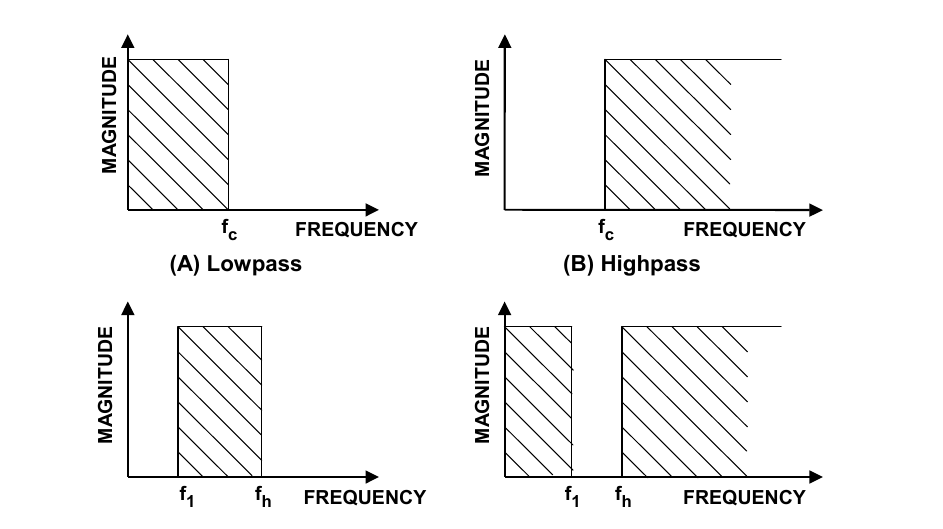
\includegraphics[width = 0.75\textwidth]{bandpass.png}
    \caption{Filter Responses (ideal)}
\end{figure} 
Passive filters are not considered here since they would not be feasable in an adjustable setup. The transfer function of a basic band-pass filter can be presented as following. 
\[
H(s) = \frac{H_0 (\omega_0)^2}{s^2 + \frac{\omega_0}{Q} s  + (\omega_0)^2}    
\]

Now let us examine briefly transfer responses in the literature to choose an optimum design path.
\subsubsection{Butterworth}
Butterworth transfer response offers clean pass and not-pass regions in other words no ripple. However, the band that allows the signals is not narrow.
\subsubsection{Chebyshev}
Chebyshev transfer response offers narrower band however it has ripples in the pass band.
\subsubsection{Bessel}
Bessel filter is optimized to obtain better transient response due to a linear phase (i.e.
constant delay) in the passband.

\vspace{4mm}
For our case as long as it is tuned carefully all three transfer responses can be used. However in order to have  better frequency discrimination Chebyshev function is selected to be used in this phase of the project. The values for the Chebyshev function will be fetched from the design tables available in internet. (The table is not included here in order not to excess page limit.)

\vspace{4mm}
Now let us examine briefly the available design topologies to choose which design path to go for. There are three main topologies for the  band-pass filter design.

\subsubsection{Multiple Feedback Band Pass}
Multiple feedback band-pass filter designs are widely used (over sallen-key filter) however does not offer much tunability. (\href{https://www.analog.com/media/en/training-seminars/tutorials/mt-220.pdf}{Source})

\subsubsection{State Variable Filter}

This configuration offers the most precise implementation
of the filter function, at the expense of many more circuit
elements. All three major parameters (gain, Q, and \(\omega_0\)) can be adjusted independently, and low-pass, high-pass, and band-pass outputs are available simultaneously. Note that the low-pass and high-pass outputs are inverted in phase while the band-pass output maintains the phase. (\href{https://www.analog.com/media/en/training-seminars/tutorials/MT-223.pdf}{Source})

\subsubsection{Dual Amplifier Band Pass}

The dual amplifier band-pass filter structure is useful in designs requiring high Qs and high frequencies. Its component sensitivity is small, and the element spread is low. A useful feature of this circuit is that the Q and resonant frequency can be adjusted more or less independently. (\href{https://www.analog.com/media/en/training-seminars/tutorials/MT-209.pdf}{Source})

\vspace{2mm}
So, it can be said that both state variable filter and dual amplifier band pass filter is quite suitable for our purposes. In this stage of the project dual amplifier band pass filter topology is selected in order to have less components. Now let us examine general outlook of the topology.
\begin{figure}[H]
    \centering
    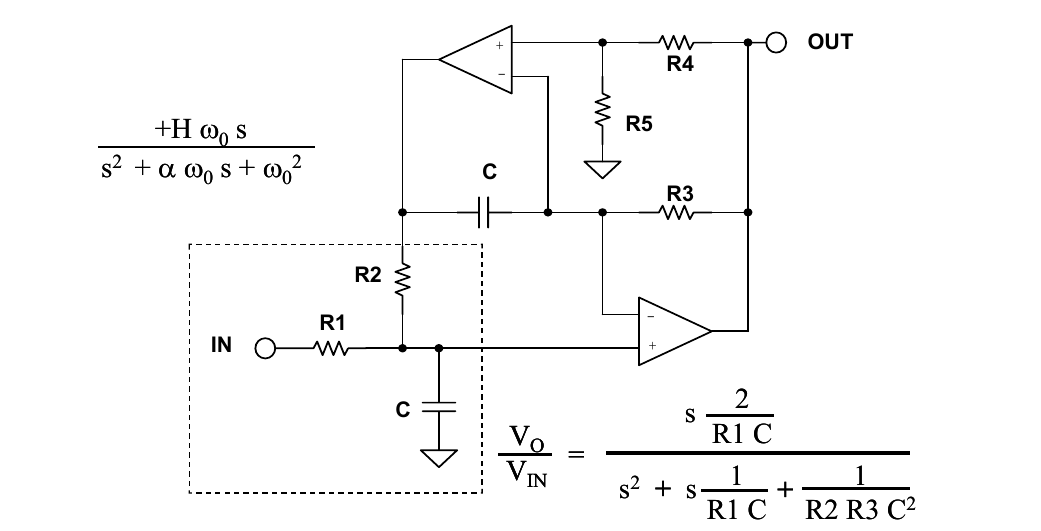
\includegraphics[width = 0.75\textwidth]{dualbandpass.png}
    \caption{Dual Band-Pass Topology}
\end{figure} 
In Figure X the in and out charactherictics also provided. In order to be able to adjust all the range of the needed frequencies, the target frequency for the base design is selected as 7kHz. With the adjustment of safety factor of 1.5 seperation is targeted as 15dB. The resulting (targeted) curve is obtained as given in Figure X.
\begin{figure}[H]
    \centering
    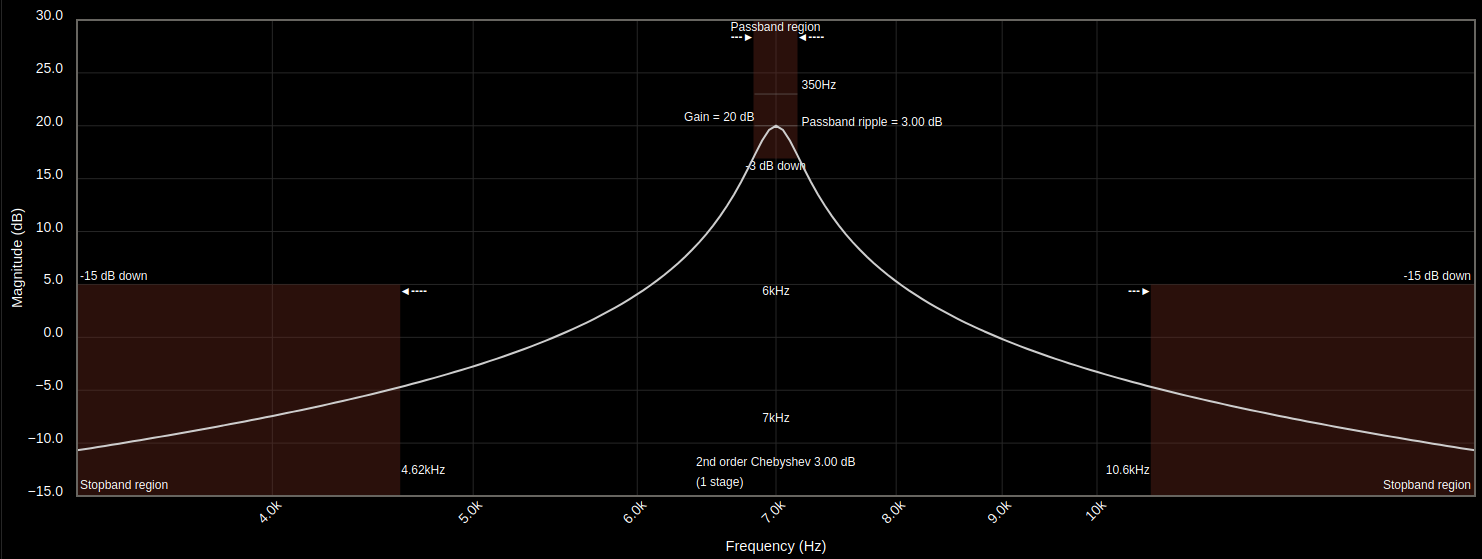
\includegraphics[width = 0.75\textwidth]{response.png}
    \caption{Targeted base frequency response}
\end{figure} 
To conclude the receiver unit, the trade-offs for first design steps are created according to the requirements specified. As explained the accuracy of the receiver part dependent on the multiple factors such as the opamp used the Q factor aimed and so on. To avoid misleading false-positive results and preserve the length of the preliminary report no simulation results are given even though they are done. The milestones that will be done in the next phase of the project for the receiver side can be summerized as;
\begin{itemize}
    \item Filter parameters will be iteratively tuned.
    \item Opamp's for the application will selected and purchased.
    \item Input buffer will be determined in order to satisfy low input impedance asumption of the filter design.
    \item Real life tests will be conducted and the circuit parameters will be tuned further.
\end{itemize}
\subsection{Speaker Unit}

\section{Conclusion}
\section*{Appendix A}


\end{document}

%%%%%%%%%%%%%%%%%%%%%%   EXAMPLE TABLE   %%%%%%%%%%%%%%%%%%%%%%%%%%%%%%%%
\begin{table}[H]
\begin{center}
    \caption{Resistance reading by color code convention.}
    \vspace{2mm}
    \begin{tabular}{||c | c | c||} 
        \hline
        Color Order & Value & Tolerance \\ [0.5ex] 
        \hline\hline
        Brown / Black / Red / Gold & 1k\( \Omega \) & \( \% \) 5  \\ 
        \hline
        Yellow / Violet / Red / Gold & 4.7k\( \Omega \) & \( \% \) 5   \\
        \hline
        Brown / Grey / Orange / Gold & 18k\( \Omega \) & \( \% \) 5  \\ [1ex] 
        \hline
    \end{tabular}
\end{center}
\end{table}


%%%%%%%%%%%%%%%%%%%%%%   EXAMPLE IMAGE   %%%%%%%%%%%%%%%%%%%%%%%%%%%%%%%%
\begin{figure}[H]
\centering
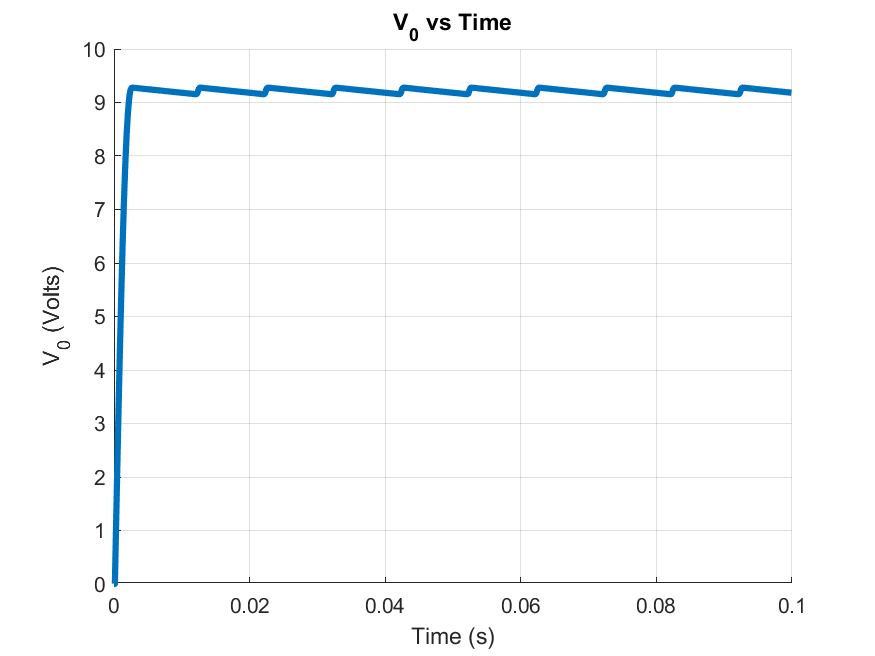
\includegraphics[width = 0.75\textwidth]{5.png}
\caption{Circuit schematic for the step 5}
\end{figure} 

%%%%%%%%%%%%%%%%%%%%%%   EXAMPLE IMAGE FROM PDF   %%%%%%%%%%%%%%%%%%%%%%%%%%%%%%%%
\begin{figure}[H] \centering{
	\includegraphics[scale=0.25]{2a_plot.pdf}}
	\caption{Experiment 2}
\end{figure}
%%%%%%%%%%%%%%%% Deneme Push